\section{Ring\-Topology Class Reference}
\label{class_ring_topology}\index{RingTopology@{RingTopology}}
Inheritance diagram for Ring\-Topology::\begin{figure}[H]
\begin{center}
\leavevmode
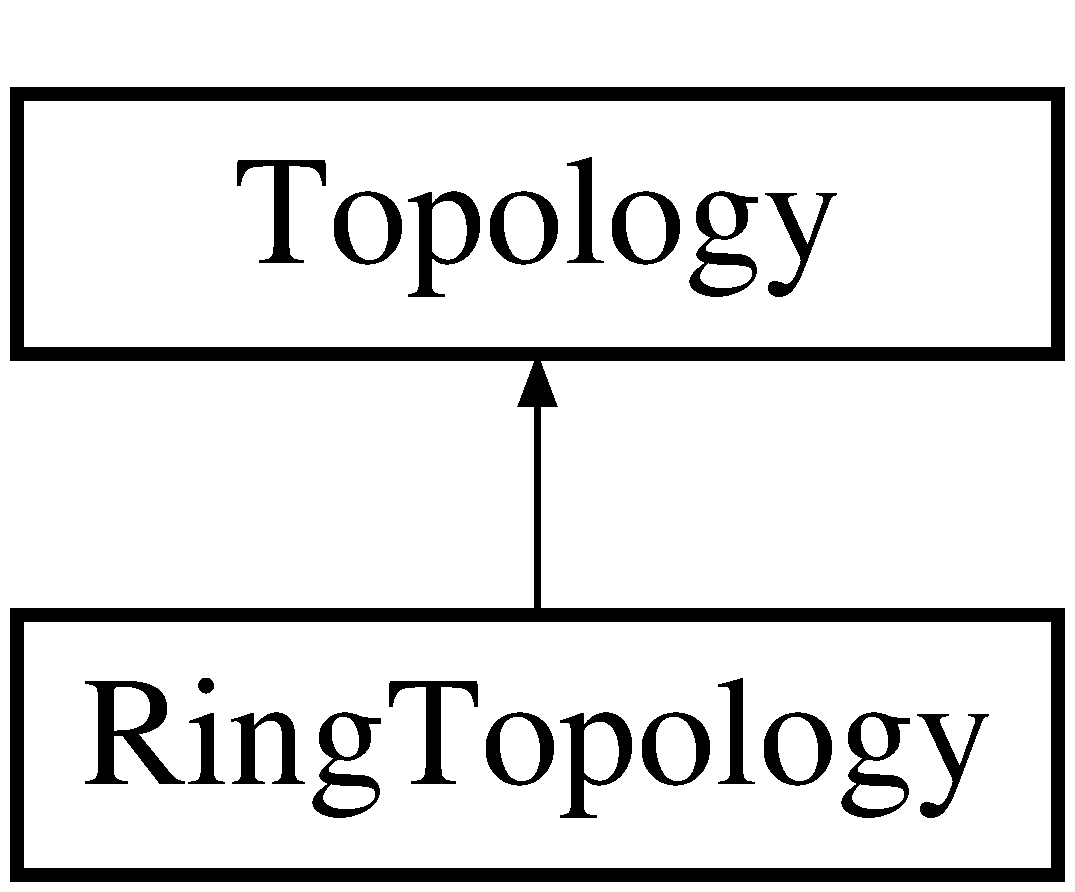
\includegraphics[height=2cm]{class_ring_topology}
\end{center}
\end{figure}
\subsection*{Public Member Functions}
\begin{CompactItemize}
\item 
void {\bf set\-Neighbors} ({\bf Cooperative} $\ast$\_\-\_\-mig, std::vector$<$ {\bf Cooperative} $\ast$ $>$ \&\_\-\_\-from, std::vector$<$ {\bf Cooperative} $\ast$ $>$ \&\_\-\_\-to)\label{class_ring_topology_292a7746993788f96042f2f628cfcbc5}

\end{CompactItemize}


\subsection{Detailed Description}




Definition at line 29 of file ring\_\-topo.h.

The documentation for this class was generated from the following files:\begin{CompactItemize}
\item 
ring\_\-topo.h\item 
ring\_\-topo.cpp\end{CompactItemize}
